\documentclass{article}
\usepackage[a4paper, top=2cm, bottom=2cm, left=2.5cm, right=2.5cm]{geometry}
\usepackage{graphicx}
\usepackage{float}
\usepackage{amsfonts}
\usepackage{amsmath}
\usepackage{listings}
\usepackage{xcolor}
\usepackage[dvipsnames]{xcolor}
\usepackage[normalem]{ulem}
\usepackage{hyperref}

\lstdefinestyle{htmlstyle}{
    language=HTML,
    backgroundcolor=\color{gray!10},
    basicstyle=\ttfamily\small,
    keywordstyle=\color{blue},
    tagstyle=\color{black},
    stringstyle=\color{green!60!black},
    commentstyle=\color{gray},
    numbers=left,
    numberstyle=\tiny\color{gray},
    stepnumber=1,
    numbersep=5pt,
    breaklines=true,
    tabsize=2,
    showstringspaces=false
}

\lstdefinelanguage{JavaScript}{
  keywords={typeof, new, true, false, catch, function, return, null, catch, switch, var, if, in, while, do, else, case, break},
  keywordstyle=\color{blue}\bfseries,
  ndkeywords={class, export, boolean, throw, implements, import, this},
  ndkeywordstyle=\color{darkgray}\bfseries,
  identifierstyle=\color{black},
  sensitive=false,
  comment=[l]{//},
  morecomment=[s]{/*}{*/},
  commentstyle=\color{purple}\ttfamily,
  stringstyle=\color{red}\ttfamily,
  morestring=[b]',
  morestring=[b]"
}

\lstset{
   language=JavaScript,
   backgroundcolor=\color{gray!10},
   extendedchars=true,
   basicstyle=\footnotesize\ttfamily,
   showstringspaces=false,
   showspaces=false,
   numbers=left,
   numberstyle=\footnotesize,
   numbersep=9pt,
   tabsize=2,
   breaklines=true,
   showtabs=false,
   captionpos=b
}

% Titolo
\title{Appunti di Linguaggi e Tecnologie per il Web}
\author{Federico Falcone}
\date{\today}

\begin{document}

\maketitle
\tableofcontents
\newpage

\section{Breakpoints}
I breakpoints sono larghezza personalizzabili che determinano come il layout responsive si comporta nei diversi dispositivi. I breakpoint predefiniti sono:
\begin{itemize}
    \item Extra small (xs): <576px
    \item Small (sm): $\geq$576px
    \item Medium (md): $\geq$768px
    \item Large (lg): $\geq$992px
    \item Extra large (xl): $\geq$1200px
    \item Extra extra large (xxl): $\geq$1400px
\end{itemize}

\section{Containers}
I container sono blocchi fondamentali che contengono e allineano il contenuto.
Bootstrap offre tre tipi di container:
\begin{itemize}
    \item .container: setta il \texttt{max-width} ad ogni rispettivo breakpoint;
    \item .container-fluid: il cui \texttt{width} é 100\% fino ad un specifico breakpoint;
    \item .container-{breakpoint}: il cui \texttt{width} è 100\% in tutti i breakpoint.
\end{itemize}
\begin{figure}[H]
    \centering
    
\includegraphics[width=1\textwidth]{Images/container.png}
\end{figure}

\section{Grid system}
Il grid system dispone 12 colonne lungo la pagina. Se non si vuole utilizzare tutte e 12 le colonne le si possono raggruppare.
\begin{figure}[H]
    \centering
    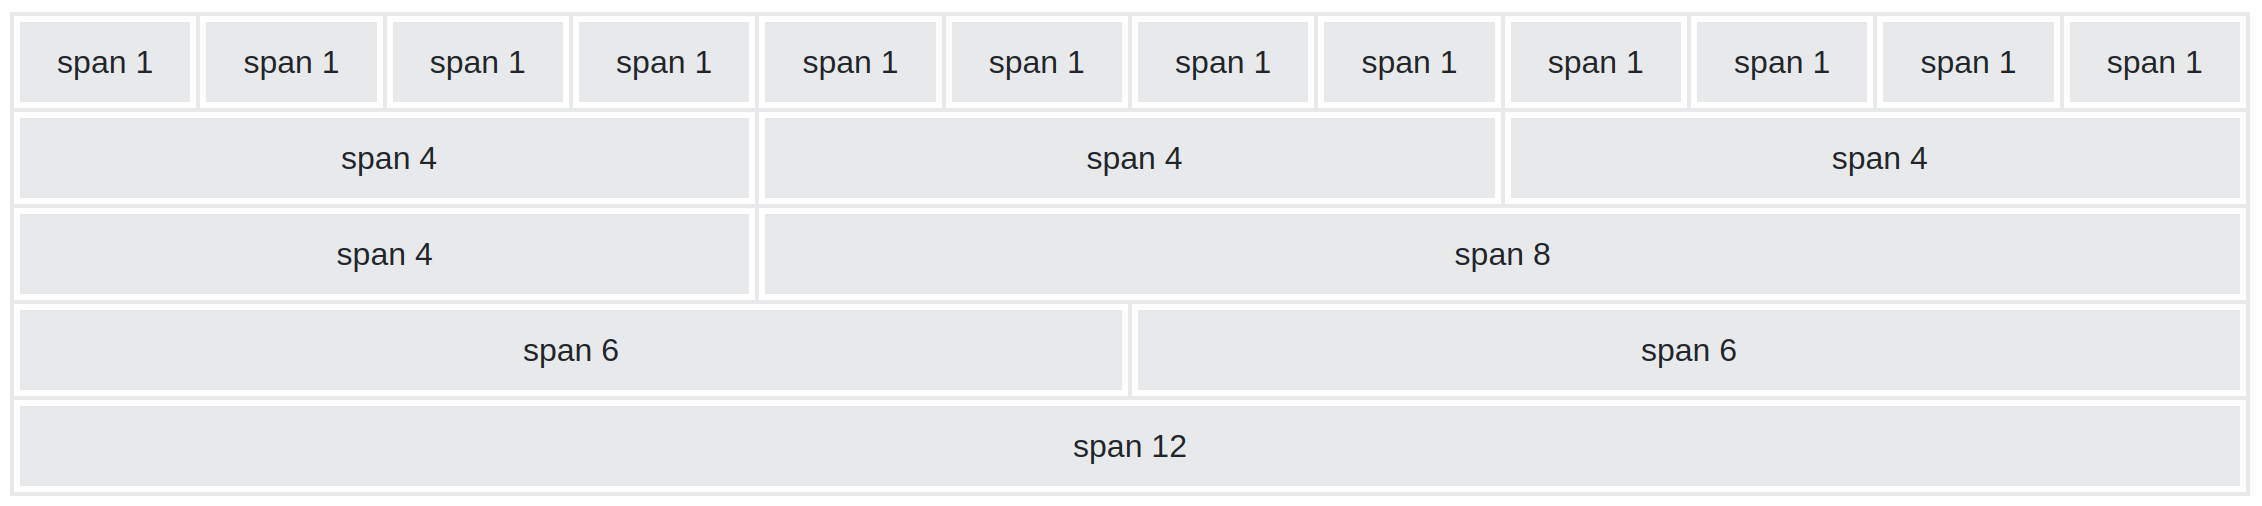
\includegraphics[width=1\textwidth]{Images/grid_system4.png}
\end{figure}
Se non utilizziamo tutte le 12 colonne, il sistema le allinea a sinistra, mentre se le superiamo andrà a capo (non lasciando lo spazio vuoto).

\section{Spacing}
Le classi per lo spacing sono composte da {property}{sides}-{breakpoint}-{size}, dove le proprietà sono:
\begin{itemize}
    \item \texttt{m} per il margine (margin);
    \item \texttt{p} per il padding.
\end{itemize}
I lati sono:
\begin{itemize}
    \item \texttt{t} setta il margine superiore (top);
    \item \texttt{b} setta il margine inferiore (bottom);
    \item \texttt{s} setta il margine sinistro (start);
    \item \texttt{e} setta il margine destro (end);
    \item \texttt{x} setta entrambi i margini orizzontali (left e right);
    \item \texttt{y} setta entrambi i margini verticali (top e bottom);
    \item vuoto per tutti e 4 i lati.
\end{itemize}
Le dimensioni sono:
\begin{itemize}
    \item \texttt{0} per classi che eliminano il margine o il padding;
    \item \texttt{1} per classi che applicano un margine o un padding di $\$spacer * 0.25$;
    \item \texttt{2} per classi che applicano un margine o un padding di $\$spacer * 0.5$;
    \item \texttt{3} per classi che applicano un margine o un padding di $\$spacer$;
    \item \texttt{4} per classi che applicano un margine o un padding di $\$spacer * 1.5$;
    \item \texttt{5} per classi che applicano un margine o un padding di $\$spacer * 3$;
    \item \texttt{auto} per classi che applicano un margine automatico.
\end{itemize}
\end{document}